\documentclass{article}
% LaTeX package to import graphics
\usepackage{graphicx}
% configuring directory path of the graphicx package
\graphicspath{{images/}}
\begin{document}
The universe is immense and it seems to be homogeneous, on a large scale, everywhere we look.

% The \includegraphcs command is provided (implemented) by the graphicx package
% it’s considered best practice to omit the file extension
% because it will prompt LATEX to search for all the supported formats.
% Generally, the graphic’s file name should not contain white spaces or multiple dots;
% it is also recommended to use lowercase letters for the file extension when uploading image files to Overleaf.
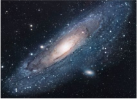
\includegraphics{universe}  
 
There's a picture of a galaxy above.

% .aux file is needed for image labelling.
% Images can be captioned, labelled and referenced by means of the figure environment.
\begin{figure}[h]
    \centering
    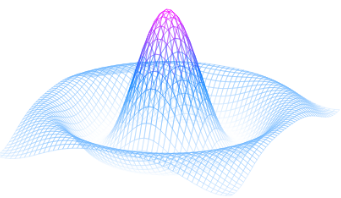
\includegraphics[width=0.75\textwidth]{mesh}
    \caption{A nice plot.}
    \label{fig:mesh1}
\end{figure} 

% Twice compilation is needed for getting the .aux file and correcting references respectively.
As you can see in figure \ref{fig:mesh1}, the function grows near the origin. This example is on page \pageref{fig:mesh1}.
\end{document}
